%###########################PRESENTACION##########################################
%Modo presentación
\documentclass[14pt]{beamer}

%Modo handout
%\documentclass[handout,compress]{beamer}
%\usepackage{pgfpages}
%\pgfpagesuselayout{4 on 1}[border shrink=1mm]

\usepackage{graphicx,pstricks}
\usepackage{beamerthemeCambridgeUS}
\usepackage{subfig}
\usepackage{tikz}
\usepackage{amsmath}
\usepackage{hyperref}

\graphicspath{{G:/My Drive/FIGURAS/}}
\setbeamercovered{transparent}

\title[GIS - Intro]{ANÁLISIS GEOESPACIAL}
\author[Edier Aristizábal]{Edier V. Aristizábal G.}
\institute{\emph{evaristizabalg@unal.edu.co}}
\date{\tiny{(Versión:\today)}}
\usepackage{textpos}

\addtobeamertemplate{headline}{}{%
	\begin{textblock*}{2mm}(.9\textwidth,0cm)
	\hfill
\includegraphics[height=1cm]{un}
	\end{textblock*}
			}
%############################INICIO#############################################
\begin{document}
\begin{frame}
\titlepage
\centering
	
\includegraphics[width=5cm]{unal}\hspace*{4.75cm}~%
   	
\includegraphics[width=2cm]{logo3}
\end{frame}
 %#############################SLIDE
\begin{frame}
\frametitle{Sistemas de Información Geográfica}
\framesubtitle{\emph {Elemento para analizar, presentar e interpretar datos espaciales}}
  \begin{figure}
    \centering
    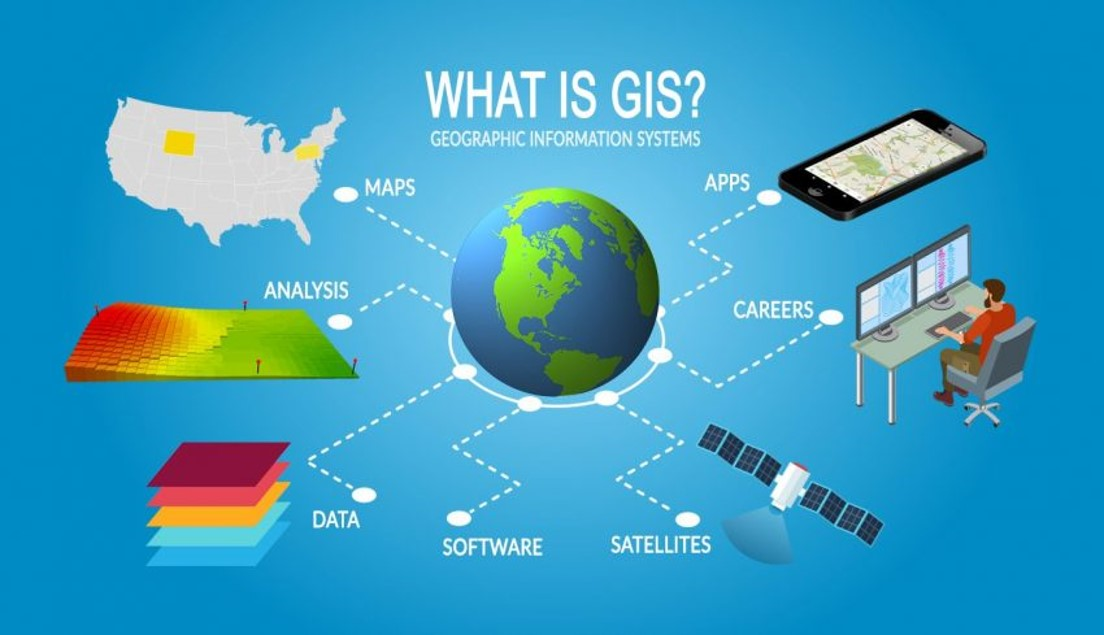
\includegraphics[height=.7\textheight]{gis}
    %\caption{This is the caption.}
  \end{figure}
\end{frame}
%################################SLIDE
\begin{frame}\frametitle{Evolución de GIS}
\begin{columns}
		\begin{column}{.48\linewidth}
			\begin{figure}
				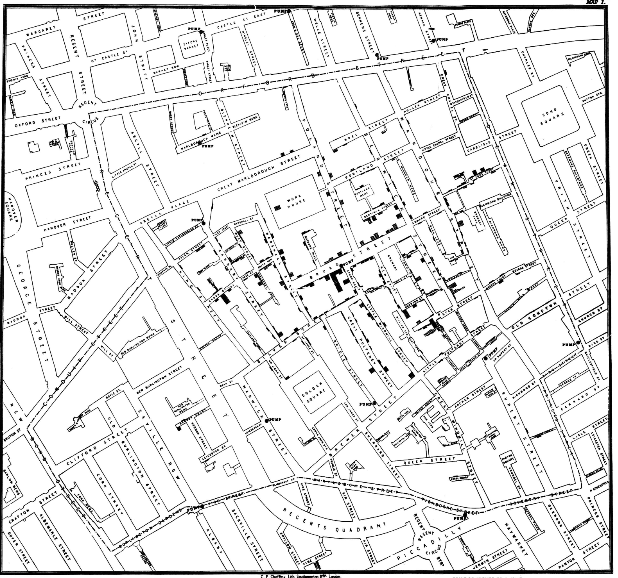
\includegraphics[width=2cm]{snow}\\
			\end{figure}
		\end{column}
		\begin{column}{.48\linewidth}
			\begin{figure}
				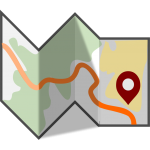
\includegraphics[width=2cm]{webgi}\\
			\end{figure}
		\end{column}
	\end{columns}
	\begin{columns}
		\begin{column}{.48\linewidth}
			\begin{figure}
				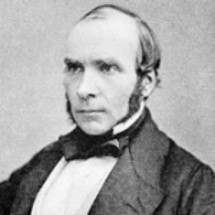
\includegraphics[width=2cm]{snow1}\\
			\end{figure}
\scriptsize{In 1854\, cholera hit the city of London, England. No one knew where the disease started. So, British physician \emph{John Snow} started mapping the outbreak. But he also mapped out roads, property boundaries and water lines.}
		\end{column}
		\begin{column}{.48\linewidth}
			\begin{figure}
				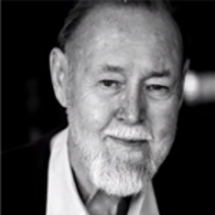
\includegraphics[width=2cm]{tomlinson}\\
			\end{figure}
\scriptsize{In 1968, \emph{Roger Tomlinson} coined the term “GIS” in his paper “A Geographic Information System for Regional Planning“. In 2014, Roger Tomlinson later passed away and will always be remembered as the \emph{father of GIS}.}
		\end{column}
	\end{columns}
\end{frame}
%###############################SLIDE
\begin{frame}
  \begin{figure}
    \centering
    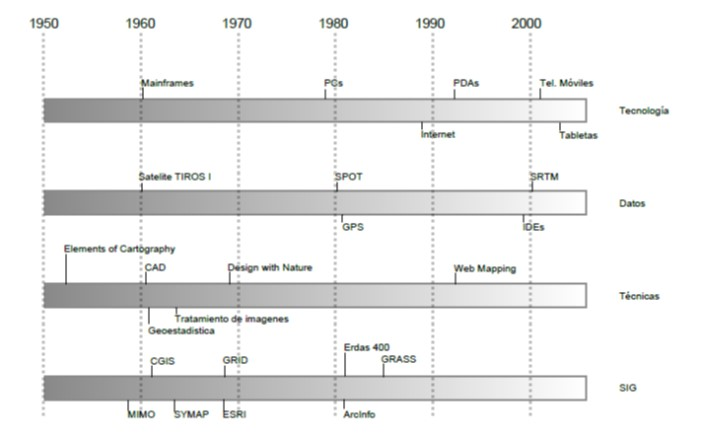
\includegraphics[height=.7\textheight]{historia}
    %\caption{This is the caption.}
  \end{figure}
\end{frame}
%################################SLIDE
\begin{frame}
\frametitle{Componentes de un SIG}
\framesubtitle{Data \& Hardware \& Software}
  \begin{figure}
    \centering
    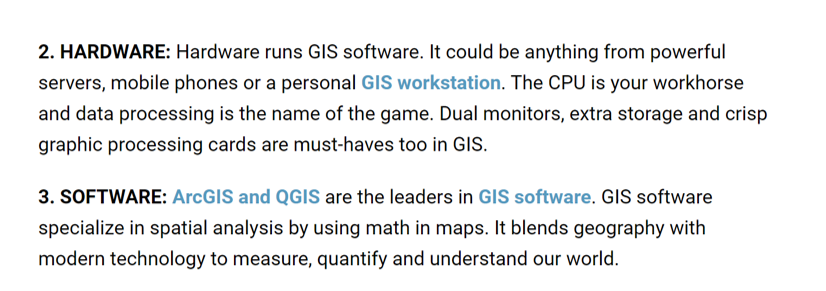
\includegraphics[width=10cm]{component2}
    %\caption{This is the caption.}
   \end{figure}
\begin{columns}
		\begin{column}{.33\linewidth}
		 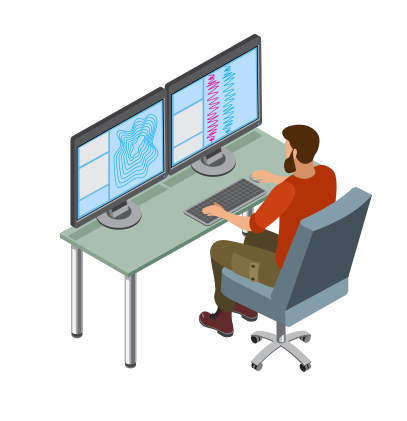
\includegraphics[height=.4\textheight]{component3}
		\end{column}
		\begin{column}{.33\linewidth}
			 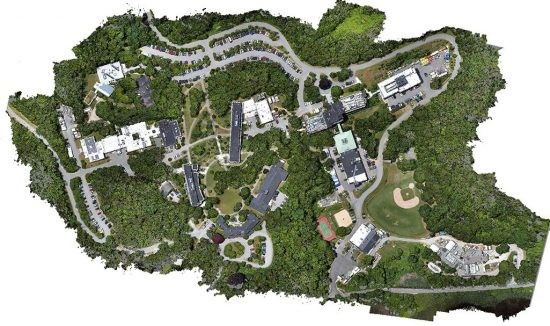
\includegraphics[height=.2\textheight]{component4}
		\end{column}
		\begin{column}{.33\linewidth}
			 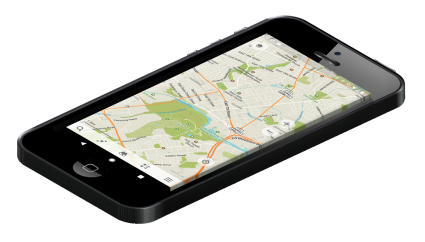
\includegraphics[height=.3\textheight]{component5}
		\end{column}
	\end{columns}
\end{frame}
%################################SLIDE
\begin{frame}
\frametitle{Hardware}
  \begin{figure}
    \centering
    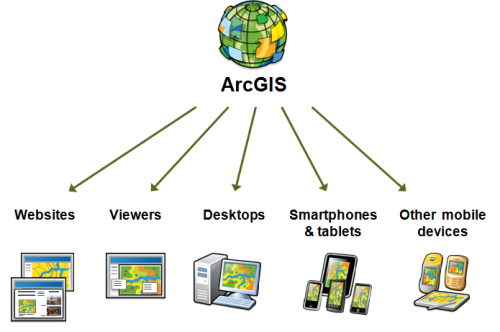
\includegraphics[height=.8\textheight]{web}
    %\caption{This is the caption.}
  \end{figure}
\end{frame}
%################################SLIDE
\begin{frame}
\frametitle{Software}
  \begin{figure}
    \centering
    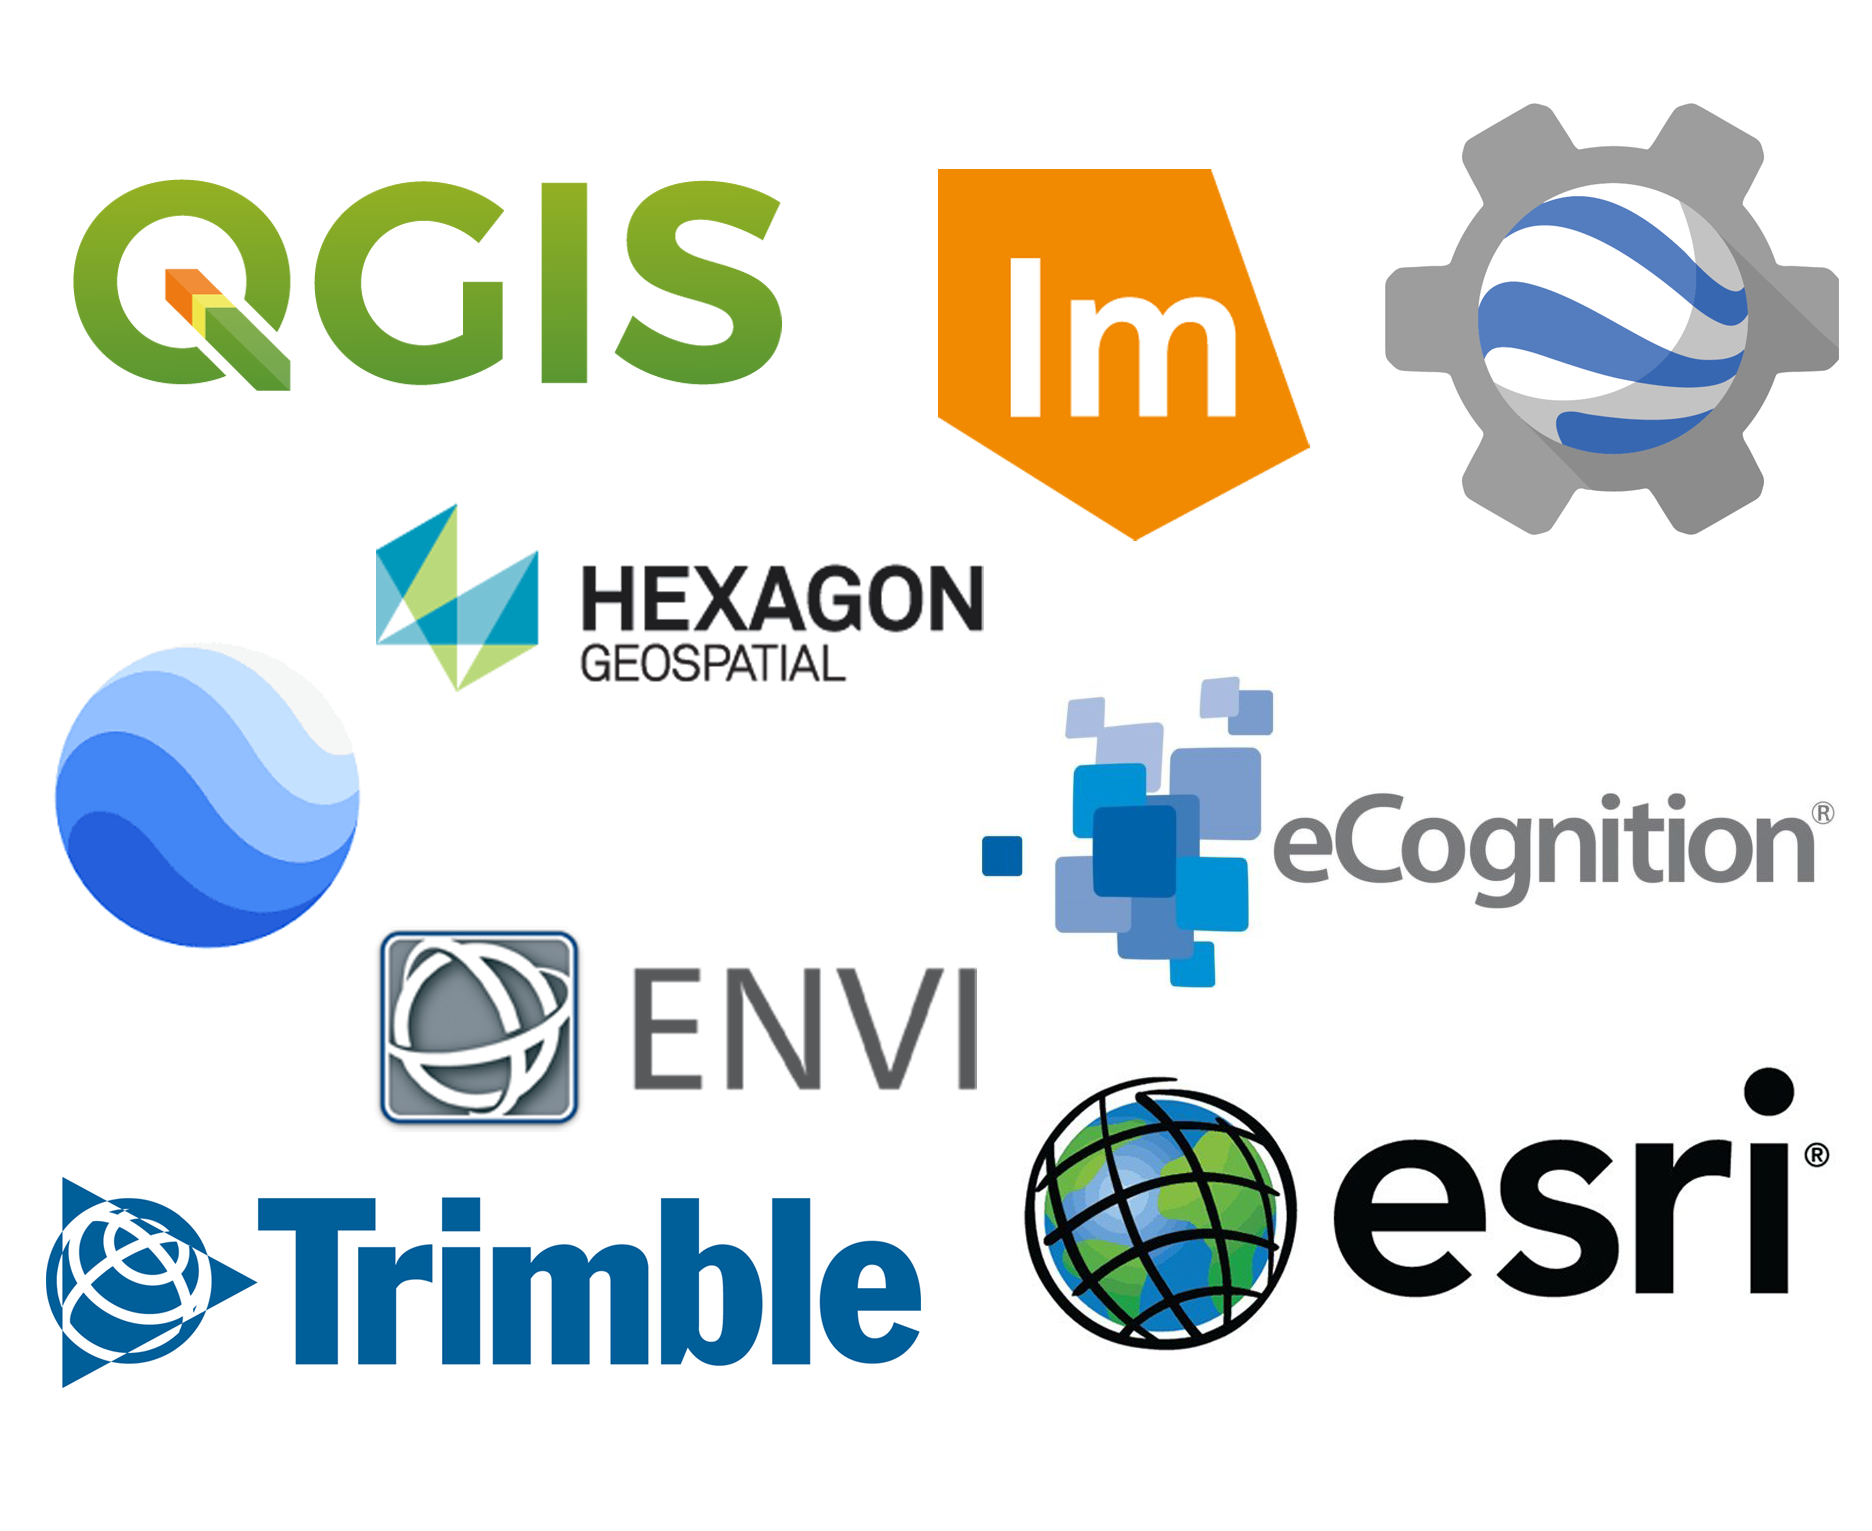
\includegraphics[height=.8\textheight]{Softwarelogos2}
    %\caption{This is the caption.}
  \end{figure}
\end{frame}
%################################SLIDE
\begin{frame}
\frametitle{Software}
  \begin{figure}
    \centering
    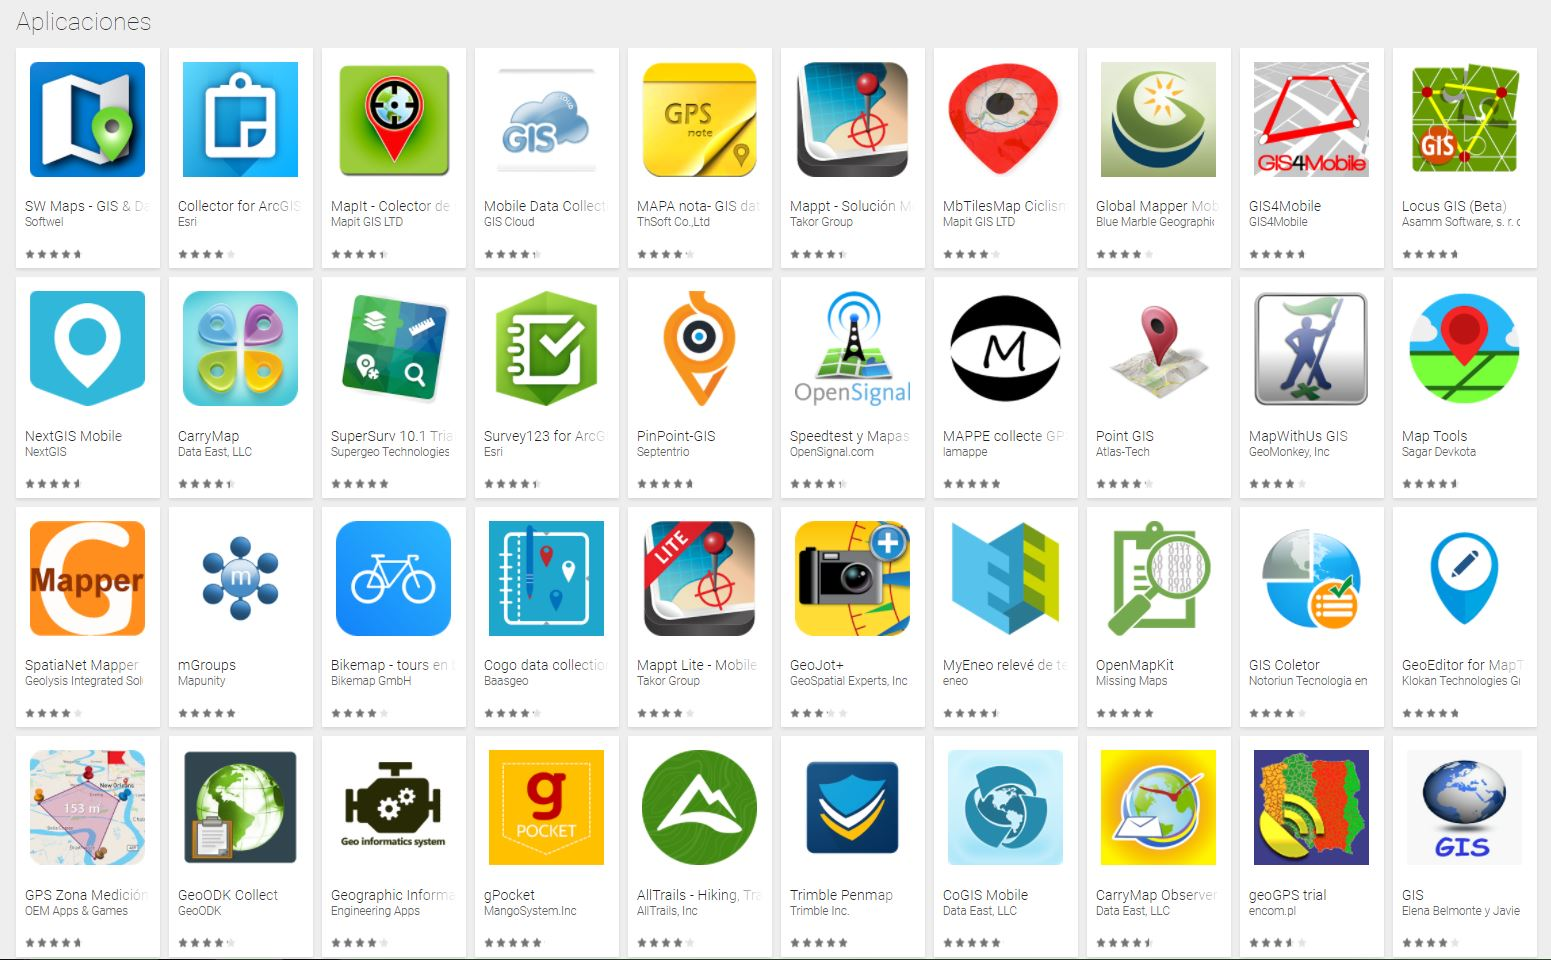
\includegraphics[height=.8\textheight]{android}
    %\caption{This is the caption.}
  \end{figure}
\end{frame}
%###############################SLIDE
\begin{frame}
\frametitle{Componentes de un SIG}
\framesubtitle{Data \& Hardware \& Software}
  \begin{figure}
    \centering
    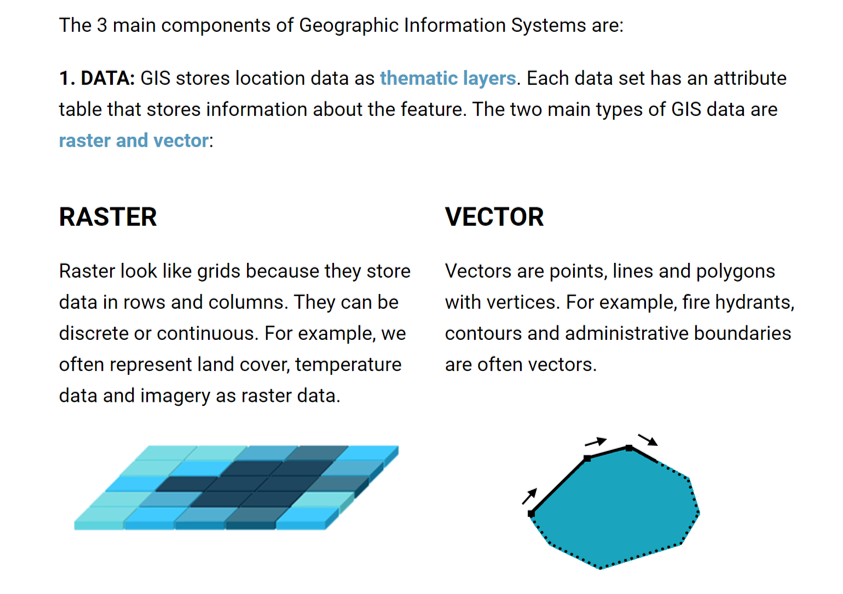
\includegraphics[height=.7\textheight]{component}
    %\caption{This is the caption.}
  \end{figure}
\end{frame}
%###############################SLIDE
\begin{frame}
\frametitle{Geospatial Data}
  \begin{figure}
    \centering
    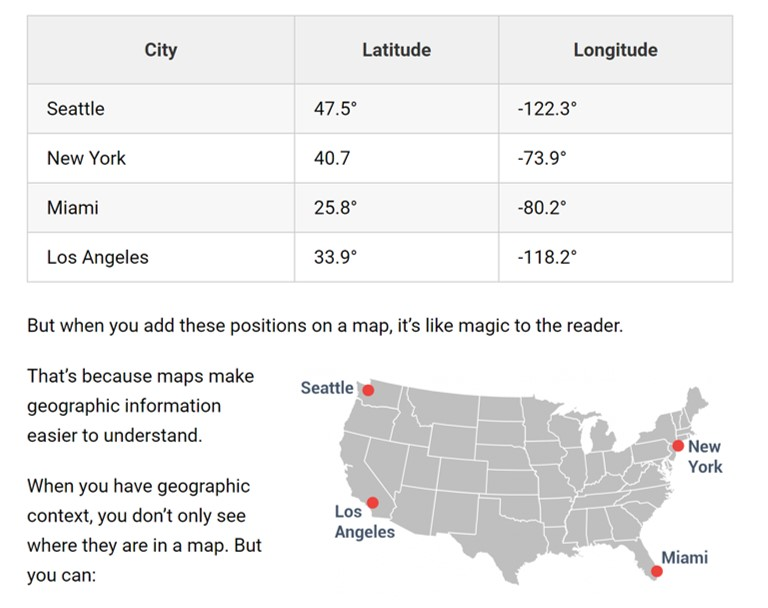
\includegraphics[height=.7\textheight]{table}
    %\caption{This is the caption.}
  \end{figure}
\end{frame}
%################################SLIDE
\begin{frame}
\frametitle{Geospatial Data}
\scriptsize{Geospatial data is data about objects, events, or phenomena that have a location on the surface of the earth, including location information (usually coordinates on the earth), attribute information (the characteristics of the object, event, or phenomena concerned), and often also temporal information (the time or life span at which the location and attributes exist).}
%\framesubtitle{}
  \begin{figure}
    \centering
    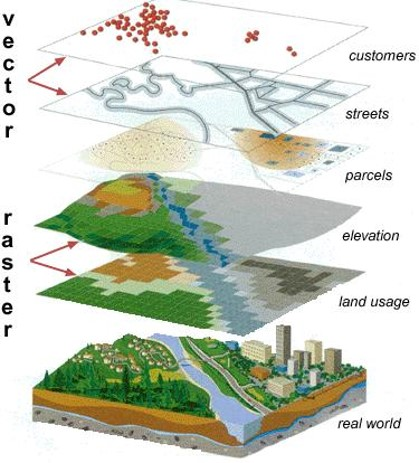
\includegraphics[height=.7\textheight]{vector}
    %\caption{This is the caption.}
  \end{figure}
\end{frame}
%################################SLIDE
\begin{frame}
\frametitle{GIS Data Models}
  \begin{figure}
    \centering
    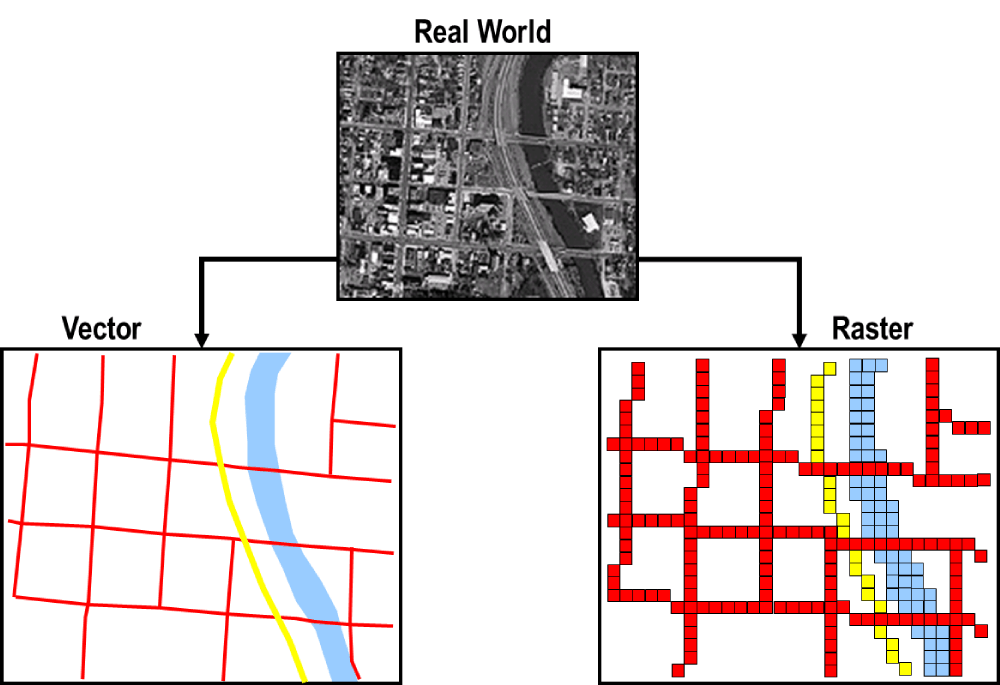
\includegraphics[height=.7\textheight]{gis_data_models}
  \end{figure}
  \tiny{\url{https://transportgeography.org/?page_id=6748}}
\end{frame}
%################################SLIDE
\begin{frame}
%\framesubtitle{}
  \begin{figure}
    \centering
    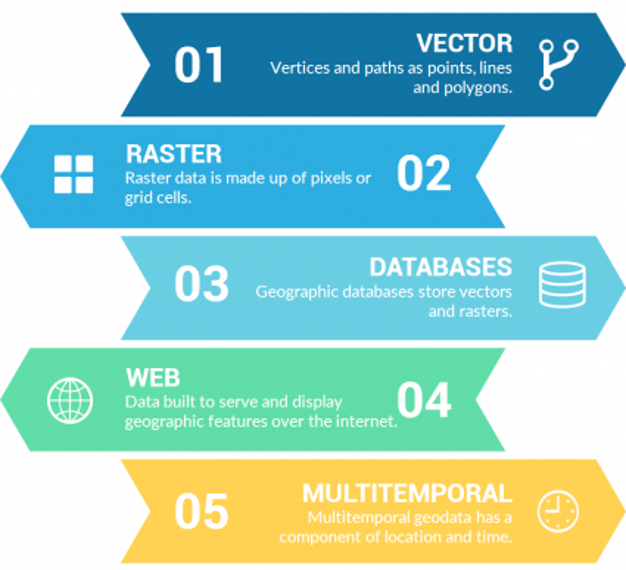
\includegraphics[height=.7\textheight]{data}
    %\caption{This is the caption.}
  \end{figure}
\end{frame}
%################################SLIDE
\begin{frame}
\frametitle{Data}
  \begin{figure}
    \centering
    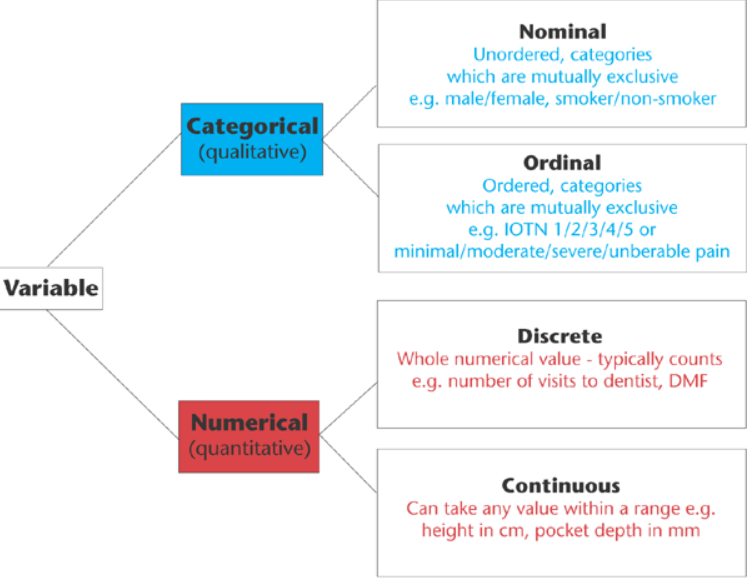
\includegraphics[height=.6\textheight]{type}
    %\caption{This is the caption.}
  \end{figure}
\end{frame}
%################################SLIDE
\begin{frame}
\frametitle{Vector}
  \begin{figure}
    \centering
    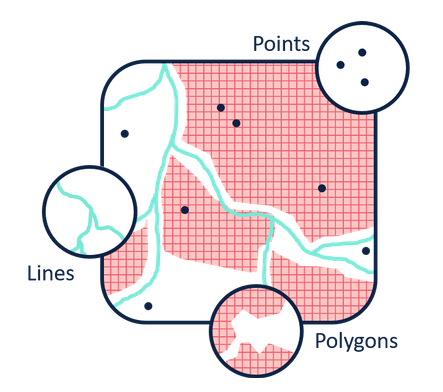
\includegraphics[height=.75\textheight]{vector_data}
  \end{figure}
\tiny{\url{https://datenlage.blog/2019/06/08/geospatial-data-1/}}
\end{frame}
%################################SLIDE
\begin{frame}
\frametitle{Vector}
  \begin{figure}
    \centering
    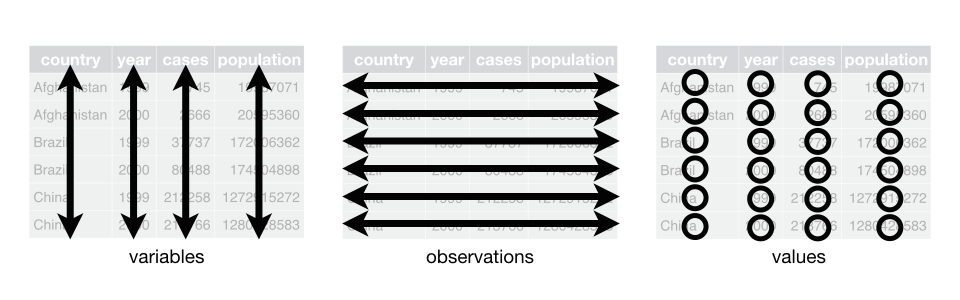
\includegraphics[height=.4\textheight]{data2}
    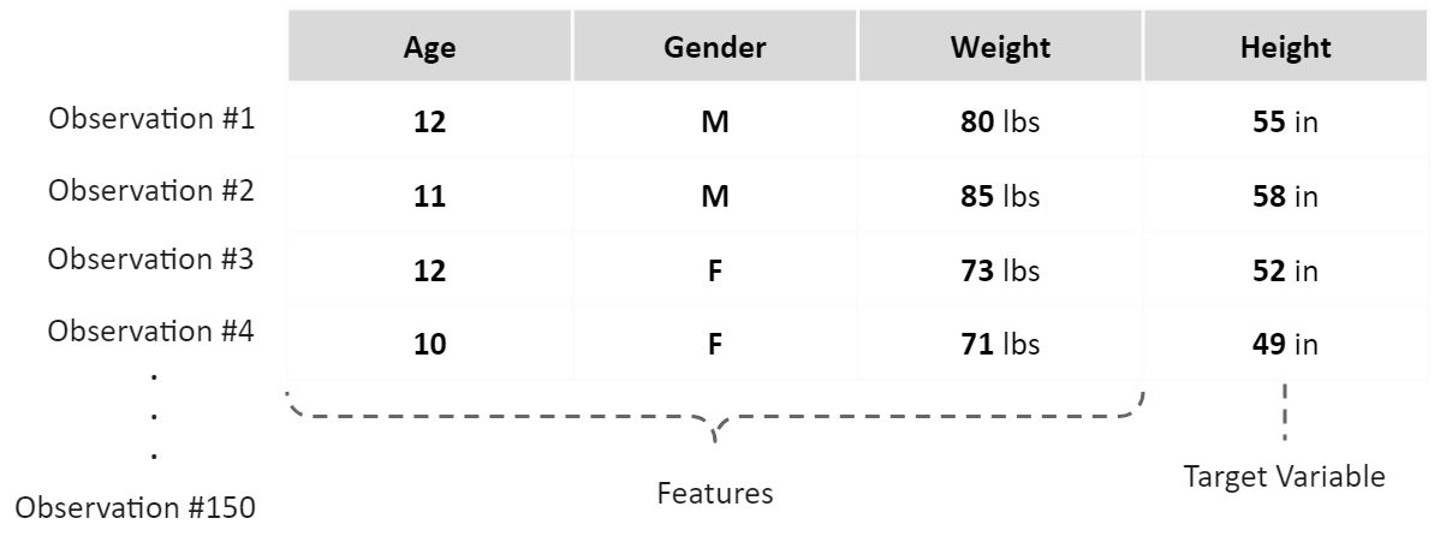
\includegraphics[height=.4\textheight]{data3}
  \end{figure}
\end{frame}
%################################SLIDE
\begin{frame}
\frametitle{Raster}
  \begin{columns}
		\begin{column}{.33\linewidth}
		 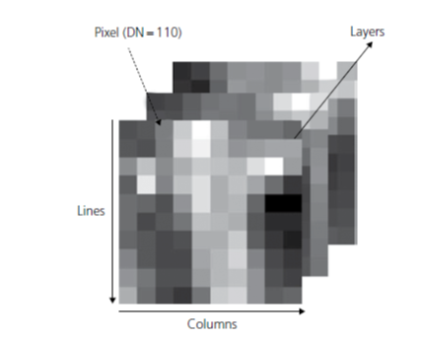
\includegraphics[height=.4\textheight]{celda}
		\end{column}
		\begin{column}{.33\linewidth}
			 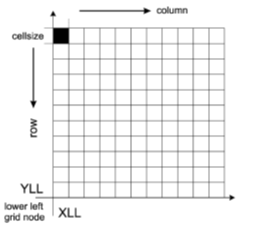
\includegraphics[height=.45\textheight]{rast2}
		\end{column}
		\begin{column}{.33\linewidth}
			 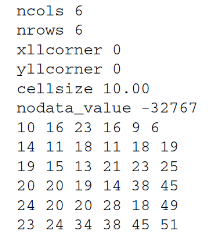
\includegraphics[height=.5\textheight]{rast3}
		\end{column}
	\end{columns}\vfill
\tiny{Wood, J. (2009). Geomorphometry - Concepts, Software, Applications. In Developments in Soil Science (Vol. 33). https://doi.org/10.1016/S0166-2481(08)00010-X}
\end{frame}
%################################SLIDE
\begin{frame}
\frametitle{Raster Continuos}
\scriptsize{Continuous rasters (non-discrete) are grid cells with gradual changing data such as elevation, temperature or an aerial photograph. A continuous raster surface can be derived from a fixed registration point. For example, digital elevation models use sea level as a registration point. Each cell represents a value above or below sea level.}
%\framesubtitle{}
  \begin{figure}
    \centering
    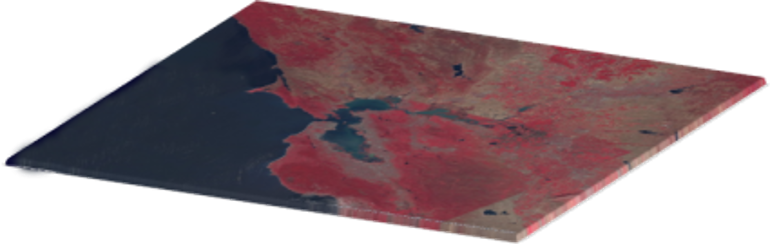
\includegraphics[height=.4\textheight]{conraster}
    %\caption{This is the caption.}
  \end{figure}
\end{frame}
%################################SLIDE
\begin{frame}
\frametitle{Raster Discretos}
\scriptsize{Discrete rasters have distinct themes or categories. For example, one grid cell represents a land cover class or a soil type.In a discrete raster land cover/use map, you can distinguish each thematic class. Each class can be discretely defined where it begins and ends. In other words, each land cover cell is definable and it fills the entire area of the cell.Discrete data usually consists of integers to represent classes.}
%\framesubtitle{}
  \begin{figure}
    \centering
    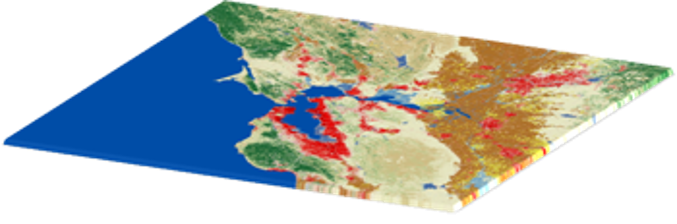
\includegraphics[height=.4\textheight]{disraster}
    %\caption{This is the caption.}
  \end{figure}
\end{frame}
%################################SLIDE
\begin{frame}
\frametitle{Formatos}
%\framesubtitle{}
%\scriptsize{}
  \begin{figure}
    \centering
    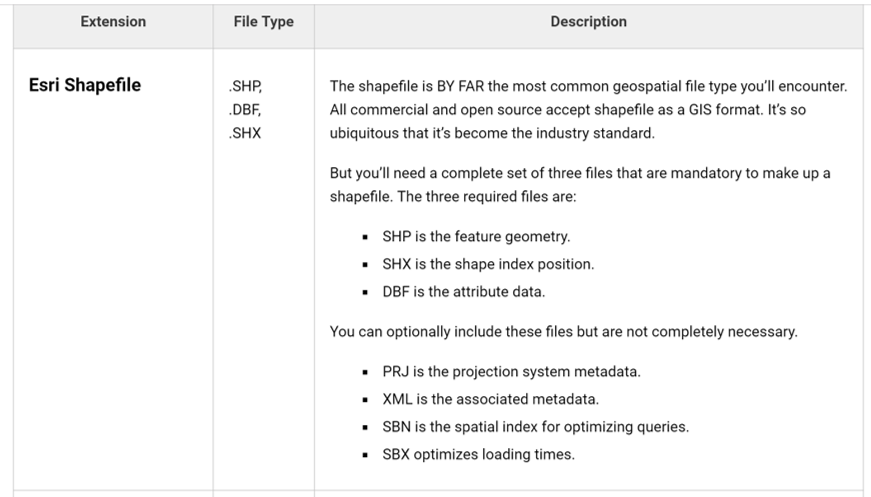
\includegraphics[height=.7\textheight]{shape}
    %\caption{This is the caption.}
  \end{figure}
\end{frame}
%################################SLIDE
\begin{frame}
\frametitle{Vector}
%\framesubtitle{}
%\scriptsize{}
  \begin{figure}
    \centering
    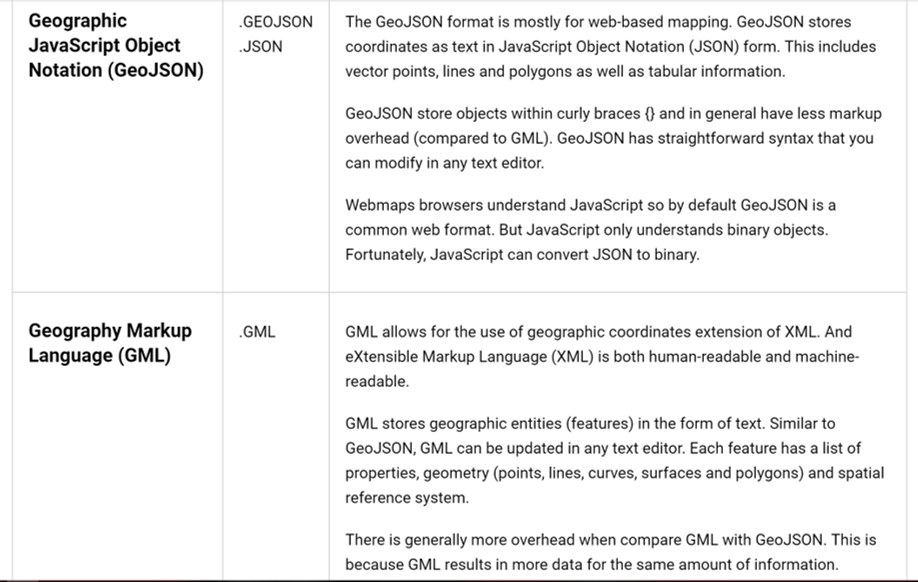
\includegraphics[height=.7\textheight]{json}
    %\caption{This is the caption.}
  \end{figure}
\end{frame}
%################################SLIDE
\begin{frame}
\frametitle{Vector}
%\framesubtitle{}
%\scriptsize{}
  \begin{figure}
    \centering
    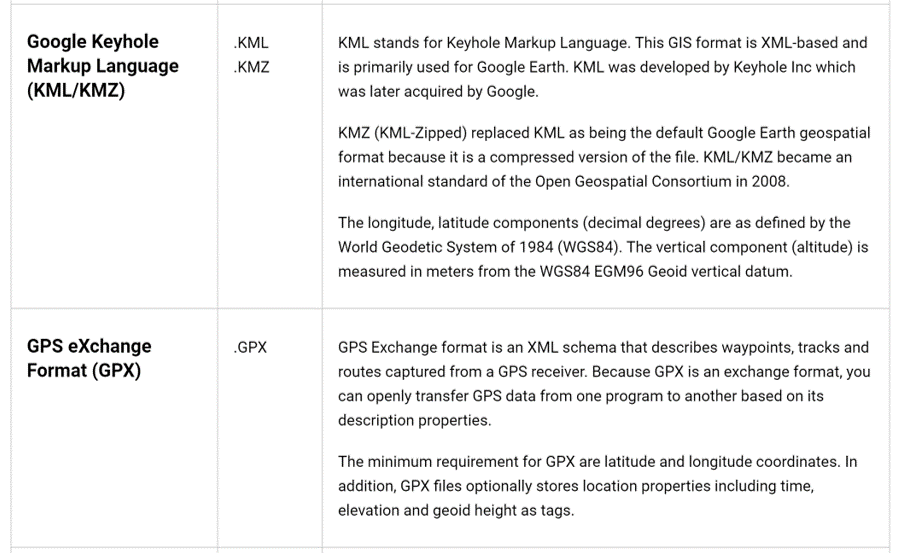
\includegraphics[height=.7\textheight]{kml}
    %\caption{This is the caption.}
  \end{figure}
\end{frame}
%################################SLIDE
\begin{frame}
\frametitle{Raster}
%\framesubtitle{}
%\scriptsize{}
  \begin{figure}
    \centering
    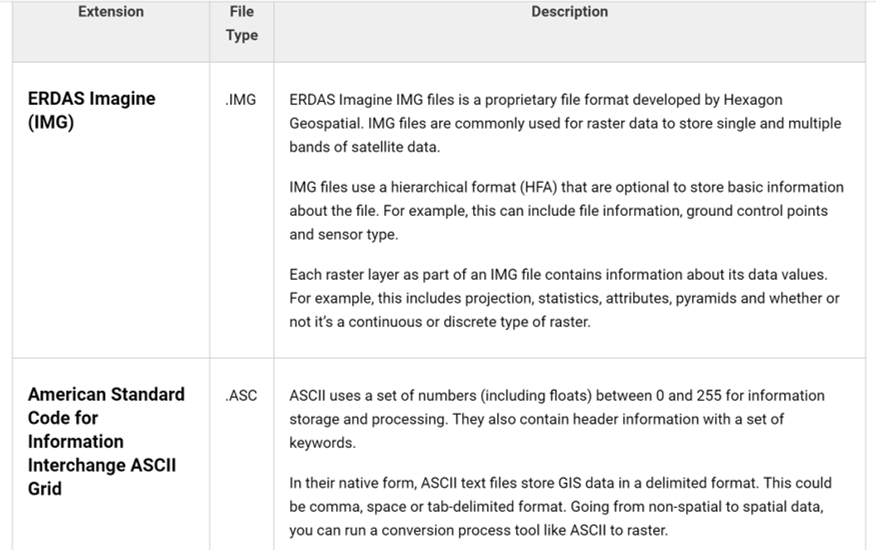
\includegraphics[height=.7\textheight]{raster}
    %\caption{This is the caption.}
  \end{figure}
\end{frame}
%################################SLIDE
\begin{frame}
\frametitle{Raster}
%\framesubtitle{}
%\scriptsize{}
  \begin{figure}
    \centering
    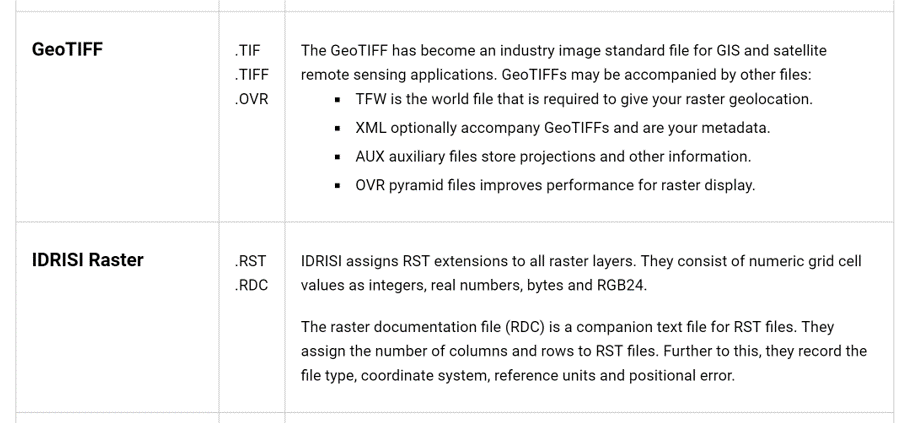
\includegraphics[height=.7\textheight]{tiff}
    %\caption{This is the caption.}
  \end{figure}
\end{frame}
%################################SLIDE
\begin{frame}
\frametitle{Raster}
%\framesubtitle{}
%\scriptsize{}
  \begin{figure}
    \centering
    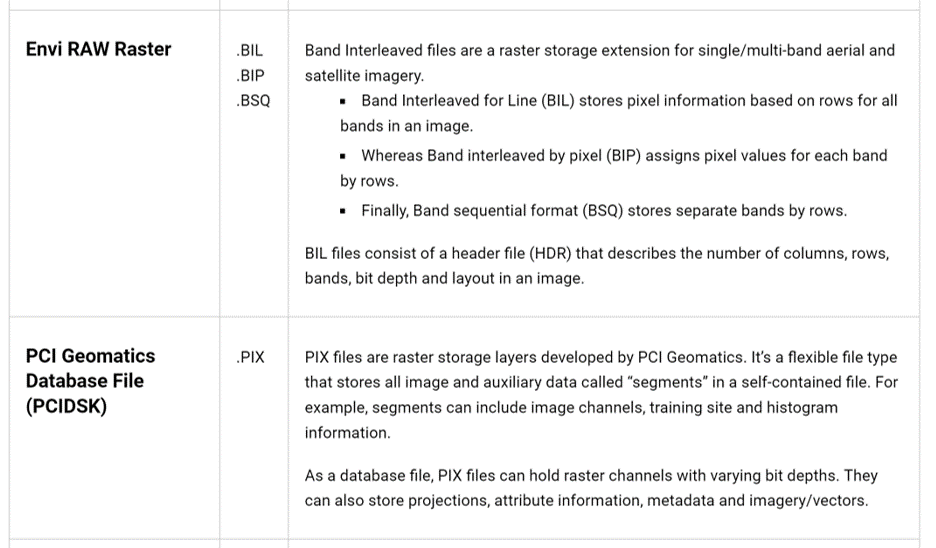
\includegraphics[height=.7\textheight]{bil}
    %\caption{This is the caption.}
  \end{figure}
\end{frame}
%################################SLIDE
\begin{frame}
\frametitle{Raster}
%\framesubtitle{}
%\scriptsize{}
  \begin{figure}
    \centering
    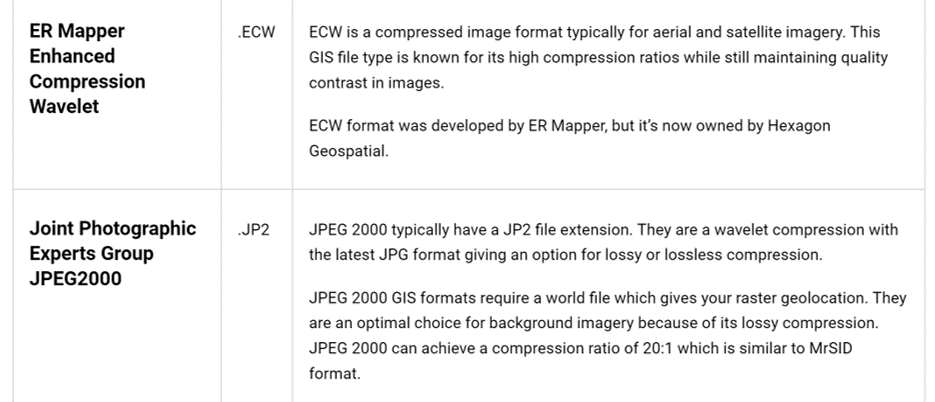
\includegraphics[height=.6\textheight]{ecw}
    %\caption{This is the caption.}
  \end{figure}
\end{frame}
%################################SLIDE
\begin{frame}
\frametitle{Raster}
%\framesubtitle{}
%\scriptsize{}
  \begin{figure}
    \centering
    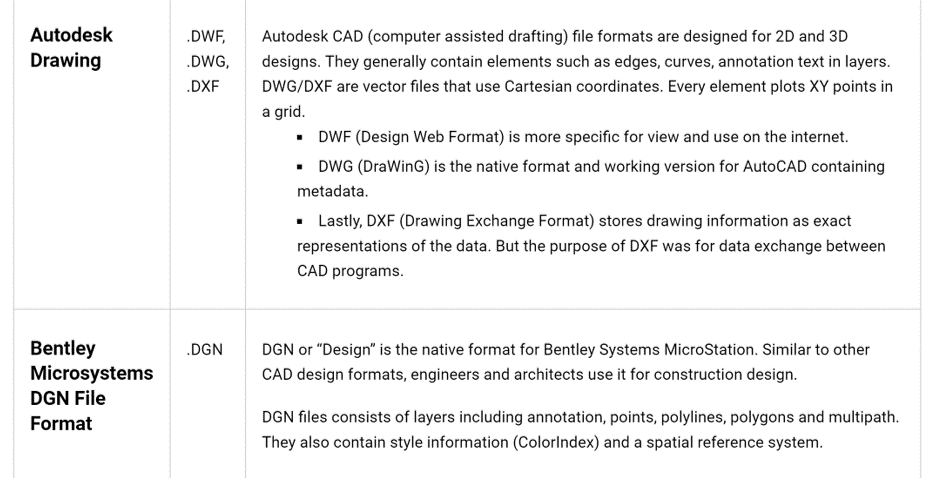
\includegraphics[height=.7\textheight]{dwg}
    %\caption{This is the caption.}
  \end{figure}
\end{frame}
%################################SLIDE
\begin{frame}
\frametitle{Raster}
%\framesubtitle{}
%\scriptsize{}
  \begin{figure}
    \centering
    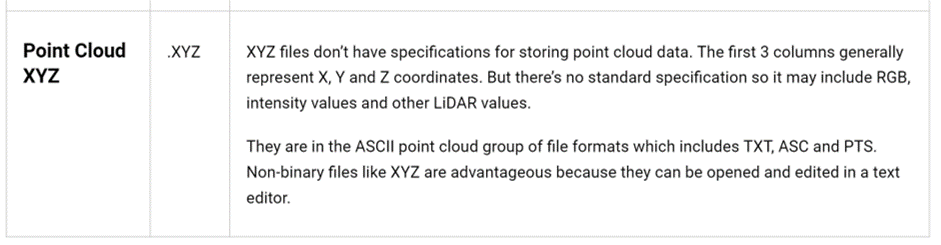
\includegraphics[height=.4\textheight]{xyz}
    %\caption{This is the caption.}
  \end{figure}
\end{frame}
%################################SLIDE
\begin{frame}
\frametitle{Raster}
%\framesubtitle{}
%\scriptsize{}
  \begin{figure}
    \centering
    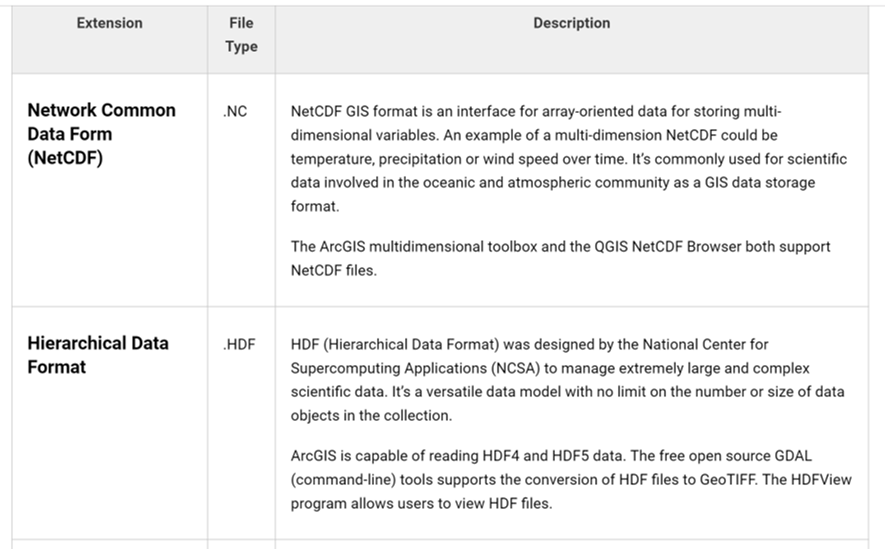
\includegraphics[height=.7\textheight]{nfc}
    %\caption{This is the caption.}
  \end{figure}
\end{frame}
%%%%%%%%%%%%%%%%%%%%%%%%%%%%%%%%%%%%%%%%%%%%%%%%%%%%%%%%%%%
\begin{frame}
\frametitle{Ejemplo}
\framesubtitle{\url{http://geojson.io/}}
%\scriptsize{}
  \begin{figure}
    \centering
    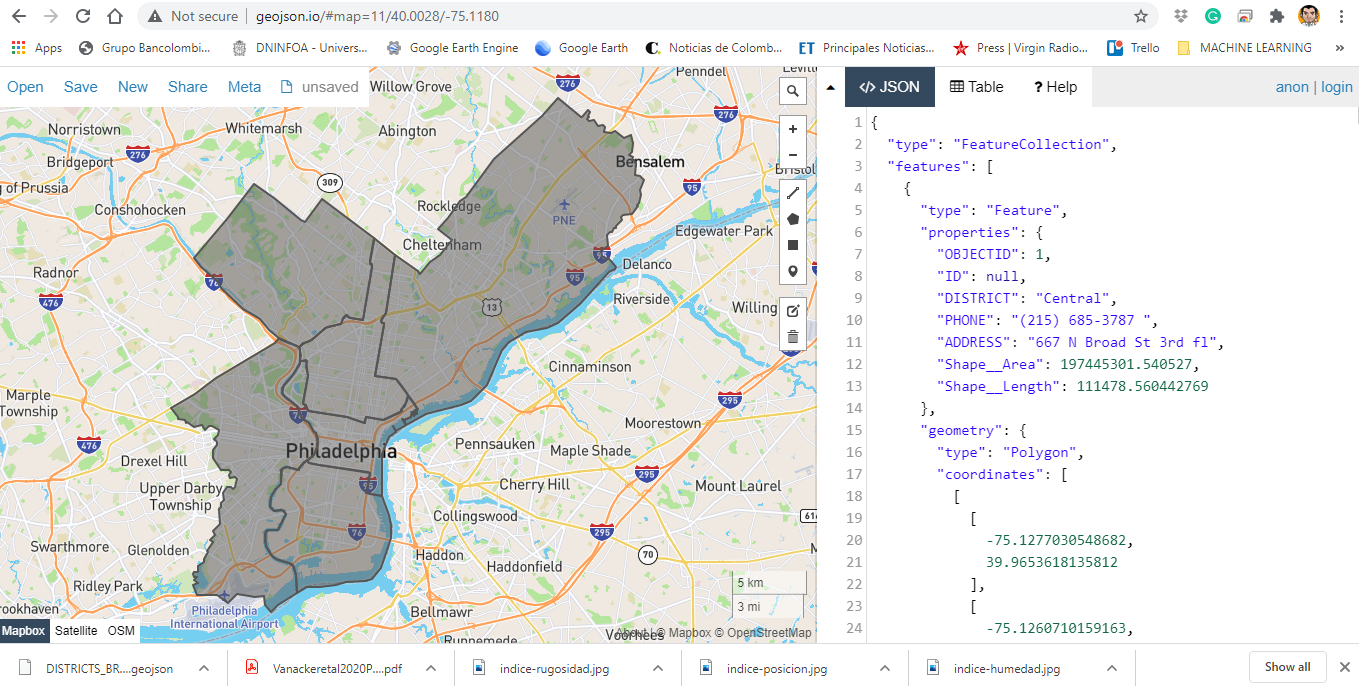
\includegraphics[height=.7\textheight]{geojson}
  \end{figure}
\end{frame}
%%%%%%%%%%%%%%%%%%%%%%%%%%%%%%%%%%%%%%%%%%%%%%%%%%%%%%%%%%%
\begin{frame}
  \frametitle{Ejemplo}
  \framesubtitle{\url{https://mapshaper.org/}}
  \begin{figure}
    \centering
    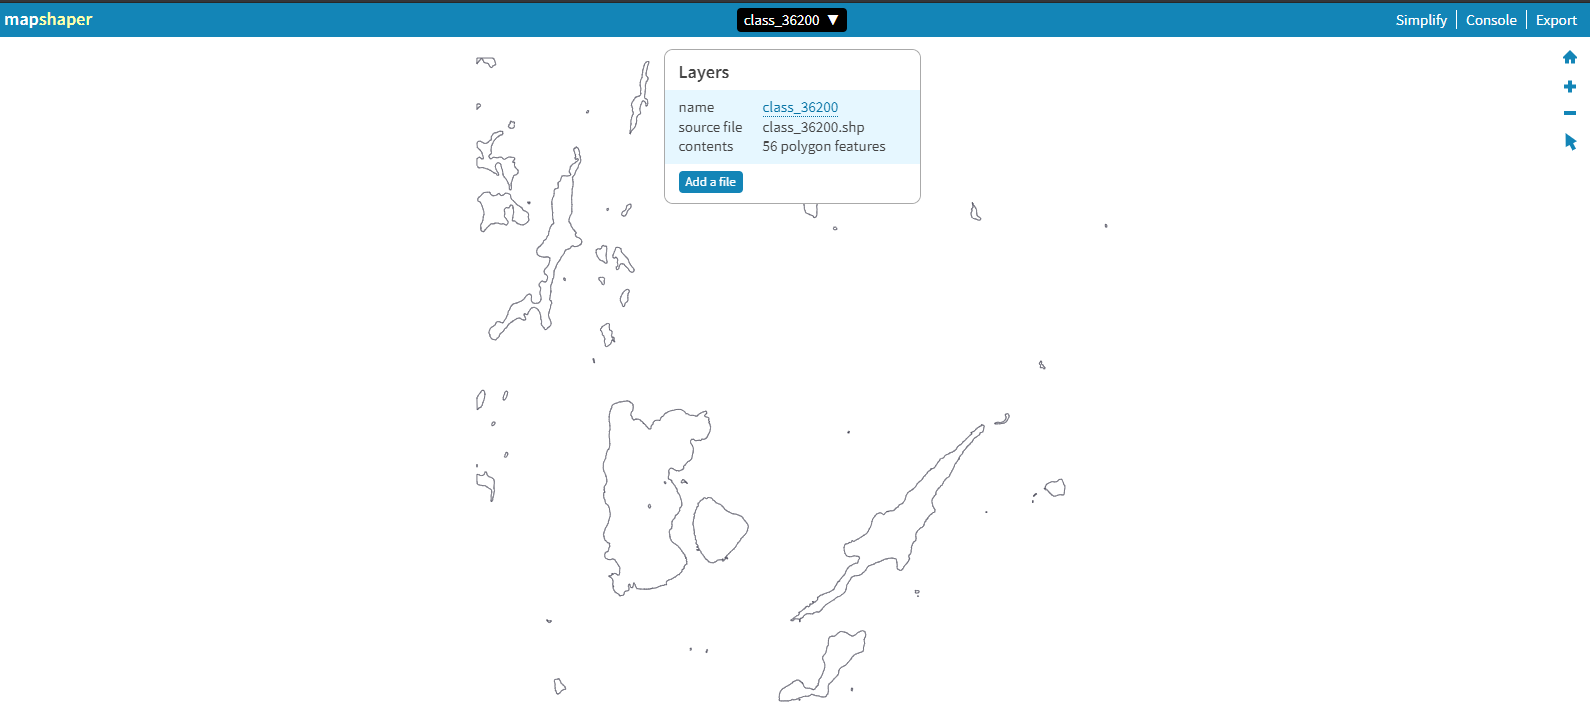
\includegraphics[height=.6\textheight]{mapshaper}\\
  \end{figure}
  \end{frame}
  %%%%%%%%%%%%%%%%%%%%%%%%%%%%%%%%%%%%%%%%%%%%%%%%%%%%%%%%%%%
\begin{frame}
\frametitle{Ejemplo}
\framesubtitle{\url{https://www.arcgis.com/home/webmap/viewer.html}}
%\scriptsize{}
  \begin{figure}
    \centering
    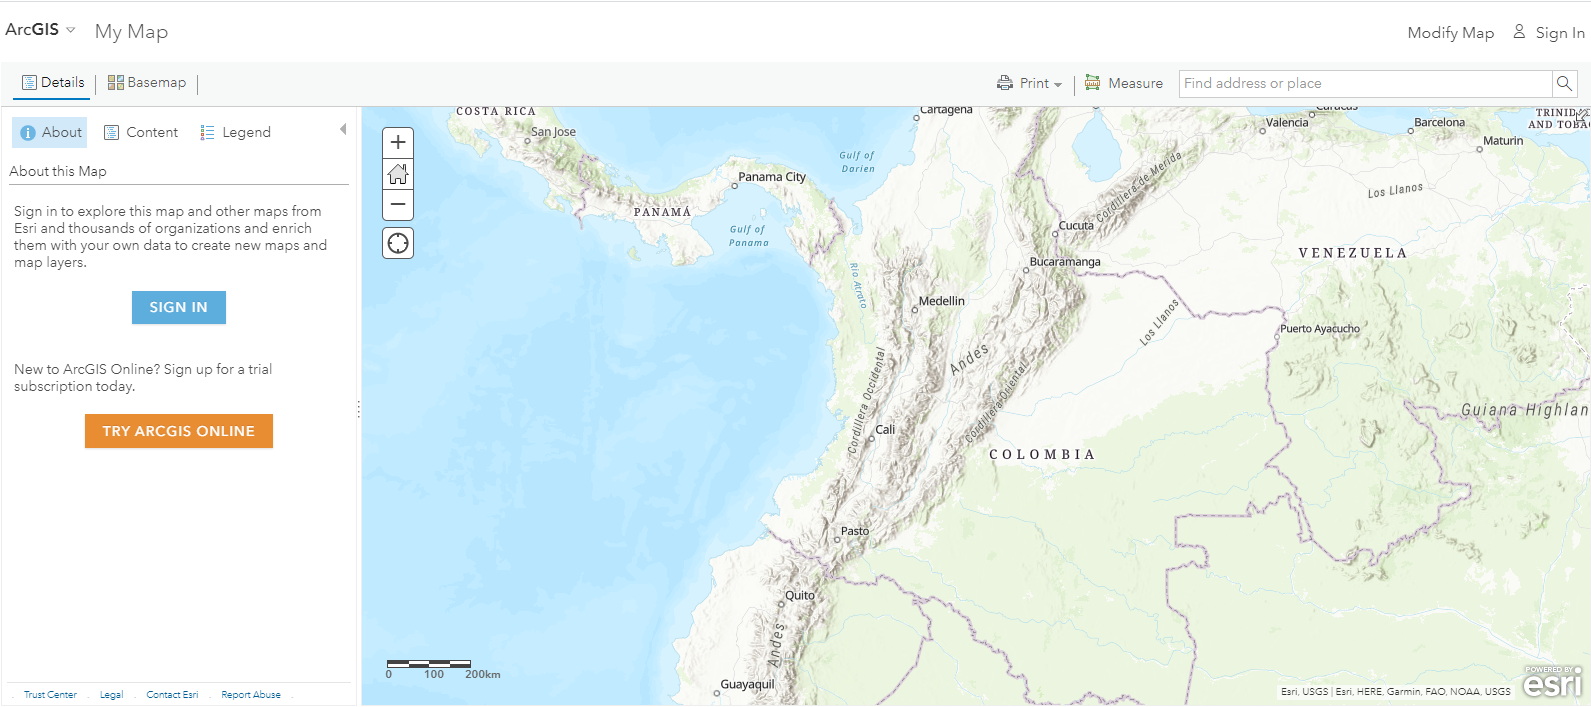
\includegraphics[height=.6\textheight]{arcgis-online}
  \end{figure}
\end{frame}
%%%%%%%%%%%%%%%%%%%%%%%%%%%%%%%%%%%%%%%%%%%%%%%%%%%%%%%%%%%
\end{document}